\section{Design}
\label{sec:design}

Roughly speaking, the conventional visualization pipeline~\cite{Card:1999} consists of two stages: the data transformation stage where data is cleaned and filtered, and the visual mapping stage where data is mapped to an appropriate visual structure (e.g., size, color). Throughout the pipeline, the user can view, navigate, and control the data states and operations, making a closed feedback loop in the interactive design.

Throughout the previous sections of this paper, we have often referred to inspiration from the computer graphics community with regards to IDE development and the use of programmable shaders.  However, this is an imprecise analogy between the visualization pipeline (Figure~\ref{fg:pipeline} (a)) and the graphics pipeline (Figure~\ref{fg:pipeline} (b)).  The graphics pipeline defines an operation flow that converts a group of vertices, textures, buffers, and states into an image~\cite{RenderMan}, while the visualization pipeline converts a wide variety of data into image.   Although the modern programmable graphics pipeline~\cite{OpenGLSL} contains multiple stages (e.g., the input assembler, the vertex shader, the hull shader, the tesselation stage, the geometry shader, the rasterizer, the pixel shader, and the output merger), its main data flow is similar to that of the fixed-function graphics pipeline: transforming the vertices and shading the fragments, which conceptually corresponds to the data transformation and visual mapping stages in the visualization pipeline.

%In the programmable graphics pipeline, the position, lighting, and texture of a primitive can be altered on-the-fly by means of algorithms and external variables or textures defined in shader programs.

The computer graphics community has had a large amount of success in utilizing programmable shaders, which is again analogous to the use of scripting languages for creating information visualizations.  In order to improve the efficiency of creating visual effects in computer graphics, textual programming editors (or IDEs) have been widely adopted in the programmable graphics pipeline~\cite{FXComposer,RenderMonkey}.  These editors provide both a visual composition component in which authors can create graphics effects from canned modules and add novel effects through programmable shaders. However, in the visualization community, existing IDEs are targeted to create visualizations without writing any code.  While this has proven effective for a variety of visualization designs, more complicated data structures and visualization effects prove difficult in the current environments.  For example, iVisDesigner~\cite{Yuan:2014:TVCG} struggles with recursive visualization structures, such as treemaps.

\begin{figure}
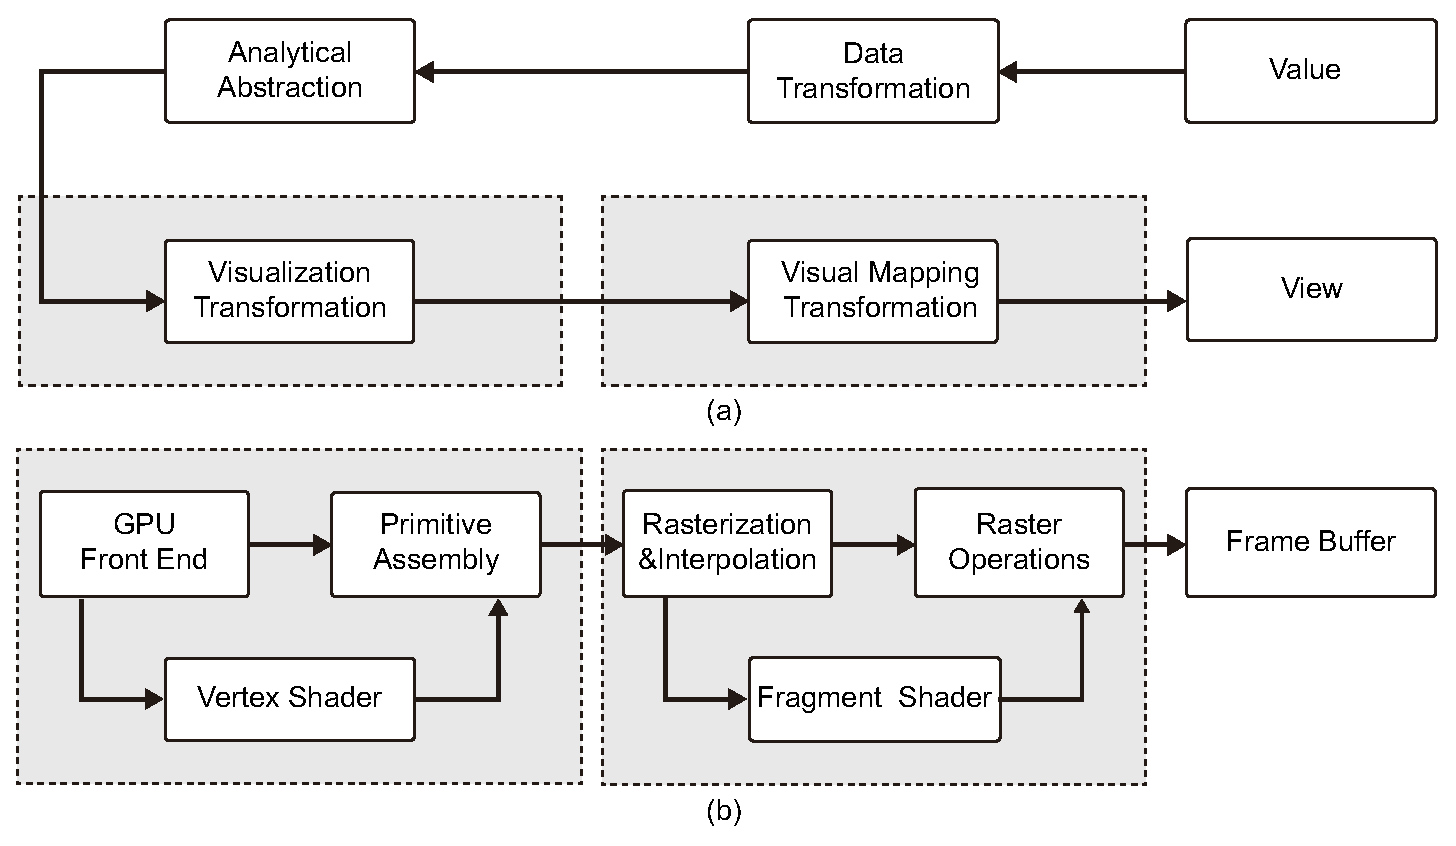
\includegraphics[width=0.99\linewidth]{images/pipelineComparison.eps}
  \caption{(a) The conventional visualization pipeline; (b) The standard graphics rendering pipeline. Both pipelines can be seen as taking a list of primitives as the input, and then mapping them from data to a visual representation.  } \label{fg:pipeline}
\end{figure}

We argue that designing a specialized visualization is analogous to the development of a shader program in terms of flexibility and expressiveness. As such VisComposer takes its cues from IDEs in the computer graphics community and can be seen as a programmable IDE for information visualizations. We introduce a new visualization composition model to support modularized management, specification and modification in designing visualizations (Section~\ref{sec:model}).  We also formulate the design of expressive visualizations as an interactive composition of visualization operations bound to selected and filtered data (Section~\ref{sec:composer}). Each operation can be exposed to the visualization authors for management, programming, and reuse, just as shaders enable programmability in the graphics pipeline.    The implemented system, VisComposer, realizes these abstractions within an integrated visual composition environment, which includes a set of control widgets, visual data views, operations and designs, and text editors (Section~\ref{sec:environment}).

We do not intend to design a visualization language. Instead, our effort is based on well-established visualization languages and toolkits and can be regarded as complementary to existing systems. %In practice, our implementation follows the visualization abstractions proposed in ProtoVis~\cite{Heer:2010:TVCG}.
